 \documentclass[a4paper,11pt,fleqn,dvipsnames,twoside,openright]{memoir} 	% Openright aabner kapitler paa hoejresider (openany begge)

%%%% PACKAGES %%%%

% ¤¤ Oversaettelse og tegnsaetning ¤¤ %
\usepackage[utf8]{inputenc}					% Input-indkodning af tegnsaet (UTF8)
\usepackage[english]{babel}					% Dokumentets sprog
\usepackage[T1]{fontenc}					% Output-indkodning af tegnsaet (T1)
\usepackage{ragged2e,anyfontsize}			% Justering af elementer
\usepackage{fixltx2e}						% Retter forskellige fejl i LaTeX-kernen

% ¤¤ Figurer og tabeller (floats) ¤¤ %
\usepackage{graphicx} 						% Haandtering af eksterne billeder (JPG, PNG, EPS, PDF)
\usepackage{epstopdf}						% Convertering af EPS til PDF (for at kunne benytte pdfLaTex
\epstopdfsetup{update}						% Only regenerate pdf files when eps file is newer
%\usepackage{eso-pic}						% Tilfoej billedekommandoer paa hver side
%\usepackage{wrapfig}						% Indsaettelse af figurer omsvoebt af tekst. \begin{wrapfigure}{Placering}{Stoerrelse}
\usepackage[space]{grffile}					% Bør gøre det muligt at have mellemrum i filnavne.
\usepackage{multirow}                		% Fletning af raekker og kolonner (\multicolumn og \multirow)
\usepackage{multicol}         	        	% Muliggoer output i spalter
\usepackage{rotating}						% Rotation af tekst med \begin{sideways}...\end{sideways}
\usepackage{colortbl} 						% Farver i tabeller (fx \columncolor og \rowcolor)
\usepackage{longtable}						% Muliggør tabeller, der strækker sig over flere sider
\usepackage{tabularx}						% Muliggør bl.a. lister/itemize indeni tabeller
\usepackage[usenames,dvipsnames]{xcolor}	% Definer farver med \definecolor. Se mere: http://en.wikibooks.org/wiki/LaTeX/Colors
%\usepackage{flafter}						% Soerger for at floats ikke optraeder i teksten foer deres reference
\let\newfloat\relax 						% Justering mellem float-pakken og memoir
\usepackage{float}							% Muliggoer eksakt placering af floats, f.eks. \begin{figure}[H]
\setlength{\heavyrulewidth}{0.15em}			% Sætter \toprule og \bottomrule til fast størrelse (0.08 er default)
%\setlength{\lightrulewidth}{0.05em}		% Sætter \midrule til fast størrelse (0.05 er default)
\usepackage{array}							% Bruges i forbindelse med \newcolumntype-command under egne commands


% ¤¤ Matematik mm. ¤¤
\usepackage{amsmath,amssymb,stmaryrd} 		% Avancerede matematik-udvidelser
\usepackage{mathtools}						% Andre matematik- og tegnudvidelser
\usepackage{textcomp}                 		% Symbol-udvidelser (f.eks. promille-tegn med \textperthousand )
\usepackage{rsphrase}						% Kemi-pakke til RS-saetninger, f.eks. \rsphrase{R1}
\usepackage[version=3]{mhchem} 				% Kemi-pakke til flot og let notation af formler, f.eks. \ce{Fe2O3}
\usepackage{siunitx}						% Flot og konsistent praesentation af tal og enheder med \si{enhed} og \SI{tal}{enhed}
\sisetup{locale=DE}							% Opsaetning af \SI (DE for komma som decimalseparator)

% ¤¤ Referencer og kilder ¤¤ %
\usepackage[danish]{varioref}				% Muliggoer bl.a. krydshenvisninger med sidetal (\vref)
\usepackage{natbib}							% Udvidelse med naturvidenskabelige citationsmodeller
\usepackage{xr-hyper}							% Referencer til eksternt dokument med \externaldocument{<NAVN>}
\externaldocument[DokRap-]{../Dokumentationsrapport/Dokumentationsrapport}	% Muliggør eksterne referencer til produktrapporten
%\usepackage{glossaries}					% Terminologi- eller symbolliste (se mere i Daleifs Latex-bog)
\usepackage{url}							% Muliggør blandt andet at indsætte url i footnote



% ¤¤ Misc. ¤¤ %
\usepackage{lipsum}							% Dummy text \lipsum[..]
\usepackage[shortlabels]{enumitem}			% Muliggoer enkelt konfiguration af lister
\usepackage{pdfpages}						% Goer det muligt at inkludere pdf-dokumenter med kommandoen \includepdf[pages={x-y}]{fil.pdf}
\pdfoptionpdfminorversion=6					% Muliggoer inkludering af pdf dokumenter, af version 1.6 og hoejere
\pretolerance=2500 							% Justering af afstand mellem ord (hoejt tal, mindre orddeling og mere luft mellem ord)

% Kommentarer og rettelser med \fxnote. Med 'final' i stedet for 'draft' udloeser hver note en error i den faerdige rapport.
\usepackage[footnote,draft,danish,silent,nomargin]{fixme}
\usepackage{listings}

%%%% CUSTOM SETTINGS %%%%

% ¤¤ Marginer ¤¤ %
\setlrmarginsandblock{3.5cm}{2.5cm}{*}		% \setlrmarginsandblock{Indbinding}{Kant}{Ratio}
\setulmarginsandblock{2.5cm}{3.0cm}{*}		% \setulmarginsandblock{Top}{Bund}{Ratio}
\checkandfixthelayout 						% Oversaetter vaerdier til brug for andre pakker

%	¤¤ Afsnitsformatering ¤¤ %
\setlength{\parindent}{0mm}           		% Stoerrelse af indryk
\setlength{\parskip}{3mm}          			% Afstand mellem afsnit ved brug af double Enter
\linespread{1,1}							% Linie afstand
\newcommand{\tab}{\hspace*{2em}}			% ved \tab{} indrykkes det i klammerne ind
\usepackage{titlesec}							%Muliiggøre ændring af sections i alle lag
\titleformat*{\section}{\LARGE\bfseries\color{NavyBlue}}		%section = størst
\titleformat*{\subsection}{\Large\bfseries\color{RoyalBlue}}		%sub = større
\titleformat*{\subsubsection}{\large\bfseries}					 %subsub = stor
\titleformat*{\paragraph}{\large\bfseries}		%Benyttes umiddelbart ikke
\titleformat*{\subparagraph}{\large\bfseries}	%Benyttes umiddelbart ikke

% ¤¤ Litteraturlisten ¤¤ %
\bibpunct[,]{[}{]}{;}{a}{,}{,} 				% Definerer de 6 parametre ved Harvard henvisning (bl.a. parantestype og seperatortegn)
\bibliographystyle{bibtex/harvard}			% Udseende af litteraturlisten.

% ¤¤ Indholdsfortegnelse ¤¤ %
\setsecnumdepth{subsubsection}		 			% Dybden af nummerede overkrifter (part/chapter/section/subsection)
\maxsecnumdepth{subsection}					% Dokumentklassens graense for nummereringsdybde
\settocdepth{subsection} 					% Dybden af indholdsfortegnelsen

% ¤¤ Lister ¤¤ %
\setlist{
  topsep=-5pt,								% Vertikal afstand mellem tekst og listen	Default: 0
  itemsep=-1ex,								% Vertikal afstand mellem items
}

% ¤¤ Visuelle referencer ¤¤ %
\usepackage[colorlinks]{hyperref}			% Danner klikbare referencer (hyperlinks) i dokumentet.
\hypersetup{colorlinks = true,				% Opsaetning af farvede hyperlinks (interne links, citeringer og URL)
    linkcolor = black,
    citecolor = black,
    urlcolor = black
}

% ¤¤ Opsaetning af figur- og tabeltekst ¤¤ %
\usepackage{caption}
\captionnamefont{\small\bfseries\itshape}	% Opsaetning af tekstdelen ('Figur' eller 'Tabel')
\captiontitlefont{\small}					% Opsaetning af nummerering
\captiondelim{. }							% Seperator mellem nummerering og figurtekst
\hangcaption								% Venstrejusterer flere-liniers figurtekst under hinanden
\captionsetup{width=\linewidth,labelfont={bf,it}}
\setlength{\abovecaptionskip}{1pt}			% Afstand over figurteksten
\setlength{\belowcaptionskip}{-12pt}			% Afstand under figurteksten

% ¤¤ Navngivning ¤¤ %
\addto\captionsdanish{
	\renewcommand\appendixname{Appendiks}
	\renewcommand\contentsname{Indholdsfortegnelse}
	\renewcommand\appendixpagename{Appendiks}
	\renewcommand\appendixtocname{Appendiks}
	\renewcommand\cftchaptername{\chaptername~}
	\renewcommand{\cftchapteraftersnum}{:} %Skriver "Kapitel xx:" foran kapitlerne i indholdsfortegnelsen
	\renewcommand\cftappendixname{\appendixname~}			% Skriver "Appendiks" foran appendiks i indholdsfortegnelsen
}

% ¤¤ Kapiteludssende ¤¤ %
\definecolor{chapnumcolor}{RGB}{23,54,93}		% Definerer en farve til brug til kapiteludseende
\definecolor{chapfontcolor}{RGB}{29,69,118}
\newif\ifchapternonum

\makechapterstyle{jenor}{					% Definerer kapiteludseende frem til ...
  \renewcommand\beforechapskip{0pt}
  \renewcommand\printchaptername{}
  \renewcommand\printchapternum{}
  \renewcommand\printchapternonum{\chapternonumtrue}
  \renewcommand\chaptitlefont{\fontfamily{pbk}\fontseries{db}\fontshape{n}\fontsize{25}{35}\selectfont\raggedleft\color{chapfontcolor}}
  \renewcommand\chapnumfont{\fontfamily{pbk}\fontseries{m}\fontshape{n}\fontsize{1in}{0in}\selectfont\color{chapnumcolor}}
  \renewcommand\printchaptertitle[1]{%
    \noindent
    \ifchapternonum
    \begin{tabularx}{\textwidth}{X}
    {\let\\\newline\chaptitlefont ##1\par}
    \end{tabularx}
    \par\vskip-2.5mm\hrule
    \else
    \begin{tabularx}{\textwidth}{Xl}
    {\parbox[b]{\linewidth}{\chaptitlefont ##1}} & \raisebox{-15pt}{\chapnumfont \thechapter}
    \end{tabularx}
    \par\vskip2mm\hrule
    \fi
  }
}											% ... her

\chapterstyle{jenor}						% Valg af kapiteludseende - Google 'memoir chapter styles' for alternativer

% ¤¤ Sidehoved ¤¤ %

\makepagestyle{AAU}							% Definerer sidehoved og sidefod udseende frem til ...
\makepsmarks{AAU}{%
	\createmark{chapter}{left}{shownumber}{}{. \ }
	\createmark{section}{right}{shownumber}{}{. \ }
	\createplainmark{toc}{both}{\contentsname}
	\createplainmark{lof}{both}{\listfigurename}
	\createplainmark{lot}{both}{\listtablename}
	\createplainmark{bib}{both}{\bibname}
	\createplainmark{index}{both}{\indexname}
	\createplainmark{glossary}{both}{\glossaryname}
}
\nouppercaseheads											% Ingen Caps oenskes

\makeevenhead{AAU}{Course 02239 - Group nr.: 02}{}{\leftmark}					% Definerer lige siders sidehoved (\makeevenhead{Navn}{Venstre}{Center}{Hoejre})
\makeoddhead{AAU}{\rightmark}{}{Ingeniørhøjskolen, Aarhus Universitet}		% Definerer ulige siders sidehoved (\makeoddhead{Navn}{Venstre}{Center}{Hoejre})
\makeevenfoot{AAU}{\thepage}{}{}							% Definerer lige siders sidefod (\makeevenfoot{Navn}{Venstre}{Center}{Hoejre})
\makeoddfoot{AAU}{}{}{\thepage}								% Definerer ulige siders sidefod (\makeoddfoot{Navn}{Venstre}{Center}{Hoejre})
\makeheadrule{AAU}{\textwidth}{0.5pt}						% Tilfoejer en streg under sidehovedets indhold
\makefootrule{AAU}{\textwidth}{0.5pt}{1mm}					% Tilfoejer en streg under sidefodens indhold

\copypagestyle{AAUchap}{AAU}								% Sidehoved for kapitelsider defineres som standardsider, men med blank sidehoved
\makeoddhead{AAUchap}{}{}{}
\makeevenhead{AAUchap}{}{}{}
\makeheadrule{AAUchap}{\textwidth}{0pt}
\aliaspagestyle{chapter}{AAUchap}							% Den ny style vaelges til at gaelde for chapters
															% ... her

\pagestyle{AAU}												% Valg af sidehoved og sidefod





%%%% CUSTOM COMMANDS %%%%

% ¤¤ Billede hack ¤¤ %
\newcommand{\figur}[4]{
		\begin{figure}[H] \centering
			\includegraphics[width=#1\textwidth]{Billeder/#2}
			\caption{#3}\label{#4}
		\end{figure}
}


% ¤¤ Venstre orienterer al tekst i p{Ycm} ¤¤ %
\newcolumntype{x}[1]{%
>{\raggedright\hspace{0pt}}p{#1}}

% ¤¤ Newline til x{} ¤¤ %
% \\ virker åbenbart ikke når man selv laver en columntype... :(
\newcommand{\tn}{\tabularnewline}


% ¤¤ Pæn opsætning af titelblad-dele ¤¤ %
% ¤¤ Husk at ændre dato i senere projekter ¤¤ %
\newcommand{\titelblad}[2]{
\begin{tabular}[ht]{x{7cm}x{7cm}}
\textbf{Navn: } #1		&\textbf{Studienummer: } #2	\tn
\textbf{Dato} 17-12-2014	\tn
\multicolumn{2}{l}{\textbf{Underskrift: }\line(1,0){340}}
\end{tabular}
}


% ¤¤ Specielle tegn ¤¤ %
\newcommand{\grader}{^{\circ}\text{C}}
\newcommand{\gr}{^{\circ}}
\newcommand{\g}{\cdot}
\newcommand{\cmark}{\ding{51}}	%Flueben
\newcommand{\xmark}{\ding{55}}	%Kryds


%%%% ORDDELING %%%%

\hyphenation{}

%%%Indsat af Søren%%%
\usepackage{listings}
\usepackage{color}

\definecolor{dkgreen}{rgb}{0,0.6,0}
\definecolor{gray}{rgb}{0.5,0.5,0.5}
\definecolor{mauve}{rgb}{0.58,0,0.82}

\lstset{ %
  language=Octave,                % the language of the code
  basicstyle=\footnotesize,           % the size of the fonts that are used for the code
  numbers=left,                   % where to put the line-numbers
  numberstyle=\tiny\color{gray},  % the style that is used for the line-numbers
  stepnumber=2,                   % the step between two line-numbers. If it's 1, each line
                                  % will be numbered
  numbersep=5pt,                  % how far the line-numbers are from the code
  backgroundcolor=\color{white},      % choose the background color. You must add \usepackage{color}
  showspaces=false,               % show spaces adding particular underscores
  showstringspaces=false,         % underline spaces within strings
  showtabs=false,                 % show tabs within strings adding particular underscores
  frame=single,                   % adds a frame around the code
  rulecolor=\color{black},        % if not set, the frame-color may be changed on line-breaks within not-black text (e.g. comments (green here))
  tabsize=2,                      % sets default tabsize to 2 spaces
  captionpos=b,                   % sets the caption-position to bottom
  breaklines=true,                % sets automatic line breaking
  breakatwhitespace=false,        % sets if automatic breaks should only happen at whitespace
  title=\lstname,                   % show the filename of files included with \lstinputlisting;
                                  % also try caption instead of title
  keywordstyle=\color{blue},          % keyword style
  commentstyle=\color{dkgreen},       % comment style
  stringstyle=\color{mauve},         % string literal style
  escapeinside={\%*}{*)},            % if you want to add LaTeX within your code
  morekeywords={*,...},              % if you want to add more keywords to the set
  deletekeywords={...}              % if you want to delete keywords from the given language
}
						% Preamble indlæses
\raggedbottom											% Sørger for at LaTeX ikke "strækker" teksten



\begin{document}										% Starter dokumentet - obligatorisk
\frontmatter											% Forindhold nummereres med romertal



% \include{Chapters/Frontpage/frontpage}
\cleardoublepage										% Indsætter tom side, så næste kapitel starter på højre side (hvis nødvendigt)



% \include{Chapters/pre_ToC/pre_ToC}						% Forindhold
\cleardoublepage


%%%% Indholdsfortegnelse (TOC) %%%%
\phantomsection											% Kunstigt afsnit, som hyperlinks kan 'holde fast i'
\pdfbookmark[0]{Indholdsfortegnelse}{indhold}			% Tildeler en klikbar bookmark til den endelige PDF
\tableofcontents*										% Indholdsfortegnelsen (kaldet ToC)



\mainmatter												% Hovedindhold - nummereres fra side 1



\chapter{Introduction}
\textcolor{red}{FROM HUBERT:\\
"This section should introduce the project and the material covered in the report. In addition, there should be an introduction to Web services (c.f. 2.1) of about roughly 2 pages."\\
Input relevant tex file(s) for introduction here...}

\section{Introduction to Web Services}
(WHAT IS IMPORTANT HERE?)
The report and implementation will introduce the concepts of web services, by implementing the Travel Agency, TravelGood, and its underlying services utilized by the agency. These underlying services are provided by other organizations, LameDuck and NiceView. These organizations provides services for TravelGood using SOAP based web service. Furthermore, all three organizations use another service, FastMoney, which is a banking system provided as SOAP based web service. See \fref{fig:BlockDiagramOverView}

% \begin{figure}[h!]
%   \caption{A picture of a gull.}
%   \centering
%     \includegraphics[width=0.5\textwidth]{gull}
% \end{figure}

\begin{figure}[h!]
\centering
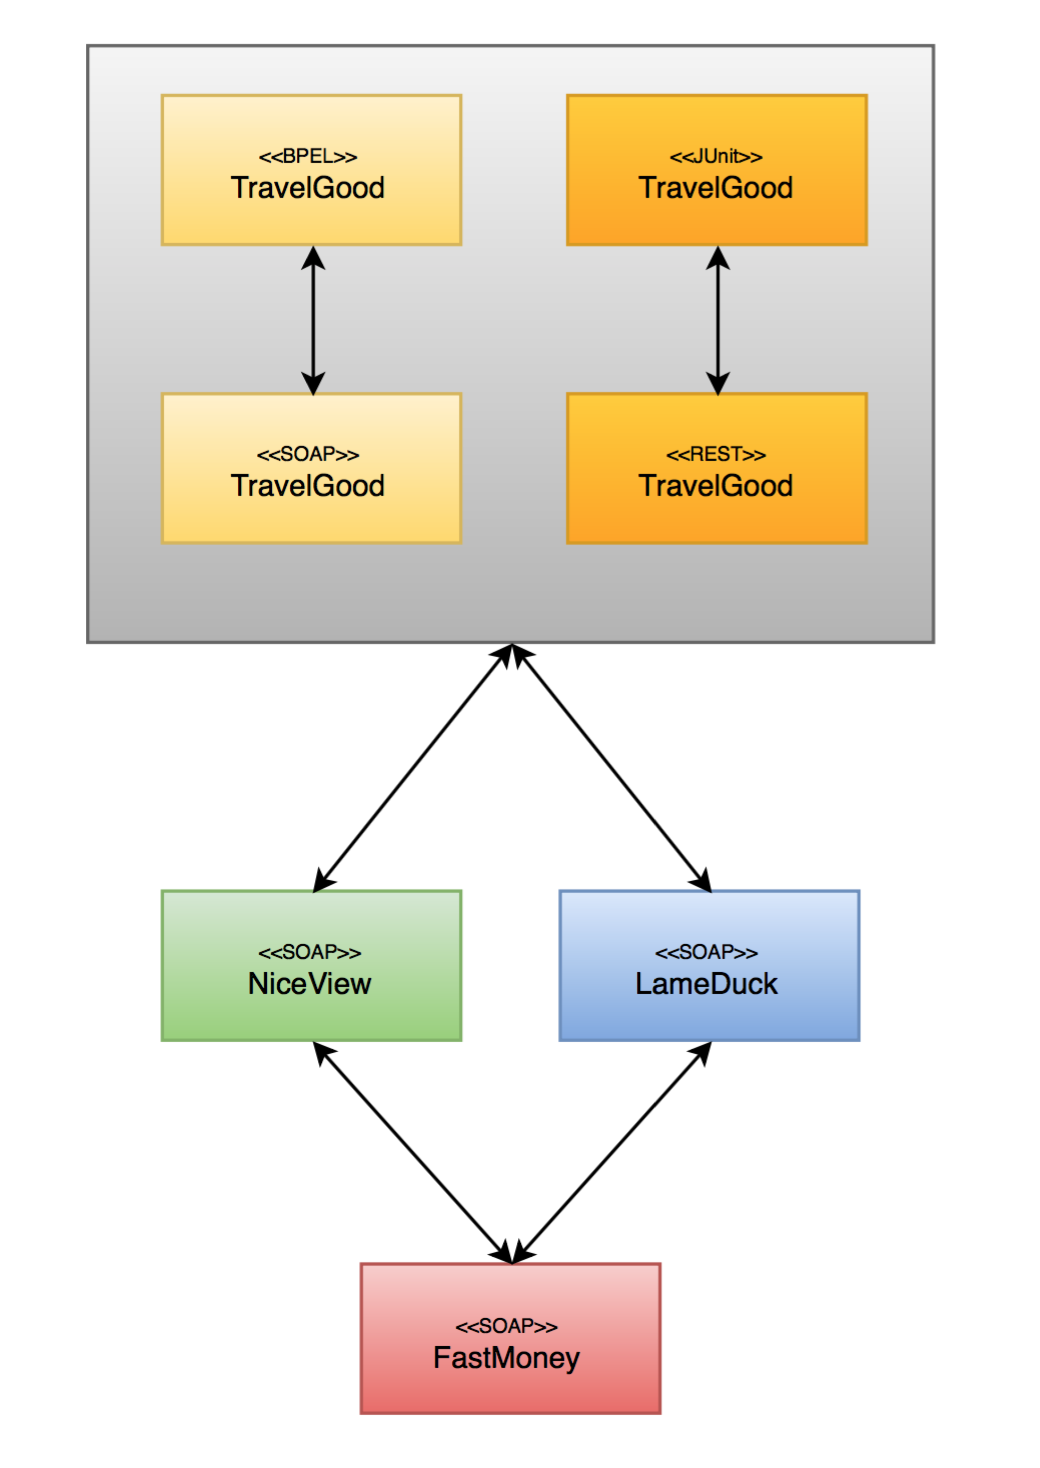
\includegraphics[width=0.4\textwidth]{Figures/BlockDiagramOverView.png}
\caption{Block Diagram - Overview}
\label{fig:BlockDiagramOverView}
\end{figure}

\subsection{Service Oriented Architecture}
\label{sub:Service Oriented Architecture}

The system utilizes SOA (Service Oriented Architecture) meaning that the systems contains several components that interacts with one another via a network using the Transport protocol, HTTP. The services are provided and described in a WSDL (Web Services Definition Language), defining the interfaces. Within the WSDL contains informations about the services/operations that can be invoked. Combined with all three services, they compose the Travel Agency service.

The Travel Agency will be implemented as both REST and SOAP based solutions, where the latter will be utilizing BPEL (Business Processing Execution Language), describing the processes that will be invoke services on NiceView and LameDuck.

\subsection{SOAP}
\label{sub:SOAP}
SOAP (Simple Object Access Protocol) is a protocol that describes how messages are exchanged on a network using HTTP as transport layer. These messages are based on XML (Extensible Markup Language) that has a set of defined rules on how these document are structured. Furthermore, a SOAP message also has a set of defined rules:

\begin{itemize}
  \item Header element that contains header information
  \item Body element that contains call and response information
  \item Fault element containing errors and status information
\end{itemize}

By being able to define the elements within a message, it introduces to strongly typed messages exchanged and messages can be sent/delivered reliably using WS-ReliableMessaging.

\subsection{BPEL}
\label{sub:BPEL}
With BPEL (Business Processing Execution Language) it is possible to describe the process of a business logic, and invoking services/operations on different web services, described in a WSDL. In another word, BPEL can be used to model the behavior of a use case, such as booking a hotel/flight.

\subsection{REST}
\label{sub:REST}
REST (Representational State Transfer) also uses HTTP protocol as its transport layer. Instead of using complex mechanism from other web services, such as SOAP, it uses simple operations from HTTP protocol that follows the CRUD (Create, Read, Update, Delete). Resources can then be accessed and execute several HTTP operations/verbs by knowing about the location of a resource in the form of URI.




% \subsection{Airline Reservation Service}
% \label{sub:Airline Reservation Service}
%
% The Airline Reservations Service, LameDuck, consists of three operations, Booking-, Cancel- and getFlights that are available for the TravelGood. LameDuck will retrieve all available flight informations from a given date. The list of informations will contain relevant informations such as departure and arrival time along with start airport and destination airport, its price and booking number.
%
% Booking of flight is handled by taking booking number and the credit card information from a given user, and upon doing so, it will validate the credit card information using FastMoney service to validate up against, for valid information and sufficient balance on the account.
%
% Lastly, cancellation is also possible in that it will cancel the booked flight, however full refund is not possible, instead a 50\% of the price will be refunded into the provided credit card information.
%
% \subsection{Hotel Reservation Service}
% \label{sub:Hotel Reservation Service}
%
% The Hotel Reservation Service, NiceView, will provide with three operations; Booking-, Cancel- and getHotels. With these operations, the service will retrieve hotel information from a given city and starting and ending date for accommodation. From these informations, NiceView will check if any rooms are available from the specified date and return a list of hotels containing available rooms and calculated price for each room.
%
% Booking of room for a given hotel is handled by taking booking number and credit card information. It checks for whether credit card is required to be validated, it will do so, calling the external web service, FastMoney.
%
% Lastly cancellation will cancel a booking by using a booking number.
%
% \subsection{Travel Agency}
% \label{sub:Travel Agency}
%
% The Travel Agency, TravelGood, will use NiceView and LameDuck and implement the business logic, as RESTful service and BPEL process. From TravelGood, it is possible to create an itinerary by booking flights and hotels for a given destination repeatedly and pay the whole itinerary by charging a credit card using FastMoney.


\chapter{Coordination Protocol}
\textcolor{red}{FROM HUBERT:\\
"This section should show and explain the state machine for the coordination protocol between the client and the travel agency – i.e. how the client is allowed to interact with the services (planning, booking, and cancelling) (c.f. 2.2)."\\
Input relevant tex files regarding Coordination Protocol here...}

\chapter{Web Service Implementations}
\textcolor{red}{FROM HUBERT:\\
"The first subsection of this section should explain the data structures used and contain class diagrams providing an overview over for the used data structures for both RESTful and SOAP/BPEL Web services The airline- and hotel reservation services mentioned in Sect. 2.3.1 and 2.3.2 should have a short description of what they do and how they are implemented. What were the design decisions involved?
For example, which binding style was used and why (e.g. document/literal)?
The next section should explain the BPEL process and how it works. It should be possible to
understand the implementation of the BPEL process from your text. Explain the design decisions you have made, e.g. what are the port types, operations, which binding style was used and why, . . . .
The last section should explain your RESTful implementation. In particular\\
• What have you chosen to be represented as resources and why\\
• How are activities of the business process mapped to HTTP verbs, like GET, PUT, POST, DELETE, . . . .\\
• How the business logic is implemented\\
• Which representations you have chosen and why"\\
Input relevant tex files regarding the implementations here...
Please create ONE tex file for each data structure used (if more than one is used).}

\section{Data Structures Used}
Write something here and input tex files for relevant subsections if any...

\section{Airline- and Hotel Reservation Services}
Write something here...

\section{BPEL Implementation}
Write something here...

\section{RESTful Implementation}
Write something qualified here... :-)


\chapter{Web Service Discovery}
\textcolor{red}{FROM HUBERT:\\
"This section should refer to, and explain the XML documents generated according to the task description in 2.6."\\
Input relevant tex files with sections on Discovery here...}

\chapter{Advaned Web Service Technology}
\textcolor{red}{FROM HUBERT:\\
"This section should discuss the points mentioned in Sect. 2.8. This section should be at most 2 pages."\\
Include files with the relevant sections here...}


\chapter{Comparison of RESTful and SOAP/BPEL Web Services}
\textcolor{red}{FROMT HUBERT:\\
"This section should discuss the points mentioned in Sect. 2.7. This section should be at most 2 pages."\\
Input necessary and relevant files with sections here...}

\chapter{Conclusion}
\textcolor{red}{FROM HUBERT:\\
"This section should summarise the report and contain the experiences with the project. For example, what was learned, what are the things you can improve next time, and what did made good this time. (Won’t be graded!)"\\
Input relevant tex files here for the conclusion...}

\chapter{Who Did What}
\textcolor{red}{FROM HUBERT:\\
"It is important that with each section/subsection it is marked who is responsible for that part of the text. There can only be one responsible person for each part of the text. In addition, each WSDL, XSD, and BPEL file needs to have an author as well as all Java files (or other programming language file) used for implementing the simple Web services. In addition, you should list which author contributed to which section and which file in the section Who did what in the report.
\textit{Make sure that each member of the group does something of each task! In particular, but not exclu- sively, make sure that all of you work on the RESTful part as well as on the SOAP/BPEL part.}"\\
Input relevant tex file about who did what parts here...}





%%%% Fixme-listen %%%%
%\newpage												% Ny side til Fixme-listen
%\listoffixmes											% Fixme-listen - udkommenteres til sidst i projektet



\end{document}											% Slutter dokumentet - obligatorisk
